% Template source: University of Florida Department of Physics, https://www.phys.ufl.edu/courses/phy4803L/sample-paper.zip

\documentclass[aps,twocolumn,secnumarabic,nobalancelastpage,amsmath,amssymb,nofootinbib,floatfix,letterpaper]{revtex4}

% Documentclass Options
    % aps, prl, rmp stand for American Physical Society, Physical Review Letters, and Reviews of Modern Physics, respectively
    % twocolumn permits two columns, of course
    % nobalancelastpage doesn't attempt to equalize the lengths of the two columns on the last page
        % as might be desired in a journal where articles follow one another closely
    % amsmath and amssymb are necessary for the subequations environment among others
    % secnumarabic identifies sections by number to aid electronic review and commentary.
    % nofootinbib forces footnotes to occur on the page where they are first referenced
        % and not in the bibliography
    % REVTeX 4 is a set of macro packages designed to be used with LaTeX 2e.
        % REVTeX is well-suited for preparing manuscripts for submission to APS journals.


\usepackage{chapterbib}    % allows a bibliography for each chapter (each labguide has it's own)
\usepackage{color}         % produces boxes or entire pages with colored backgrounds
\usepackage{graphics}      % standard graphics specifications
\usepackage[pdftex]{graphicx}      % alternative graphics specifications
\usepackage{epsf}          % old package handles encapsulated post script issues
\usepackage{bm}            % special 'bold-math' package
\usepackage{verbatim}			% for comment environment
\usepackage[colorlinks=true]{hyperref}  % this package should be added after all others
                                        % use as follows: \url{https://urldefense.proofpoint.com/v2/url?u=http-3A__web.mit.edu_8.13&d=DwICAg&c=sJ6xIWYx-zLMB3EPkvcnVg&r=D88uS55Tats-jlFQAC1XryFUYq8B7Lk3StFbXzgsiB4&m=Vjrc9Wj5n5rkIDMPJ5VsRj2GyXC3yXmN_zDHey6dVio&s=_byqsJfgO464rVIugNWFPmbBeIYfNiJcGS1fgIwc0m4&e= }

\usepackage{subcaption}
\usepackage{siunitx}
\usepackage{textcomp}
\usepackage{gensymb}
\usepackage{tikz}
\usepackage{multirow}
\usepackage{xcolor}

% Graph stuff
\usepackage[utf8]{inputenc}
\usepackage{pgfplots}
\usepgfplotslibrary{groupplots,dateplot}
\usetikzlibrary{patterns,shapes.arrows}
\pgfplotsset{compat=newest}
\usepackage{shellesc}
\usetikzlibrary{external}
\tikzexternalize

% Define colours
\definecolor{darkgreen}{HTML}{228833}

\usepackage[english]{babel}
\usepackage[autostyle, english=american]{csquotes}
\MakeOuterQuote{"}


\begin{document}
\title{Title here}
\author{Tyler Tian}
\noaffiliation
\date{\today}


\begin{abstract}
TODO
\end{abstract}

\maketitle

%%%%%%%%%%%%%%%%%%%%%%%%%%%%%%%%%%%%%%%%%%%%%%%%%%%%%%%%%%%%%%%%%%

\section{Introduction}

\begin{equation}
    \theta(t) = \theta_0 e^{-\frac{t}{\tau}}\cos\left(2\pi\frac{t}{T} + \phi_0\right)
    \label{eqn:model}
\end{equation}

\begin{equation}
    Q = \pi\frac{\tau}{T}
    \label{eqn:qfactor}
\end{equation}

%%%%%%%%%%%%%%%%%%%%%%%%%%%%%%%%%%%%%%%%%%%%%%%%%%%%%%%%%%%%%%%%%%

\section{Method}

\subsection{Pendulum Construction}

\begin{figure}[htb]
    \includegraphics[width=0.6\linewidth]{swingy.jpg}
    \caption{Swingy the pendulum.}
    \label{fig:swingy}
\end{figure}

The main support structure of the pendulum consists of two pieces of wood attached with screws.
This was chosen because the material was readily available, and could be substituted for any material of
similar size and suitable strength.

The pendulum uses a thin, braided string, specifically chosen to minimize twisting in order to prevent the bob from
spinning. The string is lightly wound around a nail, and then directed through a hole in the support board and held
in place by a binder clip. A flat measuring tape is secured parallel to the string to measure the string length. A
piece of green masking tape is put over the pivot nail to enable computer-vision based tracking.

The string is attached to a bob consisting of a small, red plastic cup, specifically chosen for its high colour contrast
against the background to enable precise vision tracking. The cup is loaded with coins to vary its weight since coins
have known masses.

\subsection{Pendulum Tracking}

\begin{figure}[htb]
    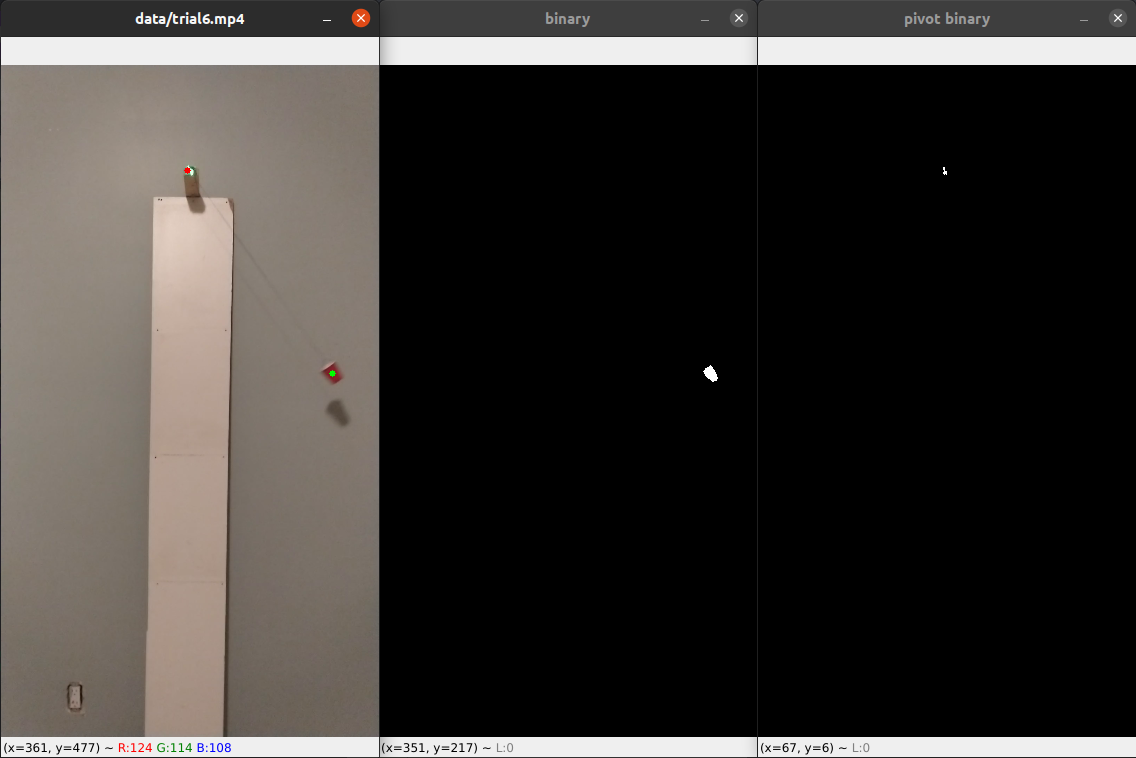
\includegraphics[width=\linewidth]{cv_track.png}
    \caption{CV-based tracking of the pendulum.}
    \label{fig:tracking}
\end{figure}

Videos of the pendulum are shot on a phone camera and then passed to a Python program written with OpenCV (see Appendix
\ref{appendix:code}). The locations of the bob and pivot are determined by thresholding the image in the HSV colour
space (the right two windows in Figure \ref{fig:tracking}), and then taking the average of the pixels that passed the
threshold to obtain the centres of the bob and pivot in the image (green and red dots in the first window in Figure
\ref{fig:tracking}). After the pixel coordinates have been determined, the ratio of the difference between the \(x\) and
\(y\) coordinates are used to compute the angle for each frame.

\subsection{Lab 1: \texorpdfstring{\(Q\)}{Q} Factor}
\label{sec:lab1_method}

For this lab, the video is shot at 60fps but only sampled at 30Hz since precise measurements are less important for
determining the \(Q\) factor. Subsequent experiments have improved this.

The string length is fixed at approximately 65cm and the mass at approximately 42g. The precise masses and lengths are
never measured as they remained constant and are unimportant for this lab.

The \(Q\) factor is obtained from the angle-time data using two independent methods:
\begin{enumerate}
    \item
        \textbf{Curve fitting:} A Python program (see Appendix \ref{appendix:code}) is used to fit the model (Equation
        \ref{eqn:model}) to the data, producing values for \(\tau\) and \(T\). \(Q\) is calculated from these values
        using Equation \ref{eqn:qfactor}.
    \item
        \textbf{Oscillation counting:} By substituting \(t = T\frac{Q}{n}\) (i.e. \(\frac{Q}{n}\) oscillations) into
        the decay term in Equation \ref{eqn:model}, the term becomes
        \begin{equation}
            \theta_0 e^{-\frac{T\frac{Q}{n}}{\tau}} = \theta_0 e^{-\frac{T\frac{\pi\frac{\tau}{T}}{n}}{\tau}} = \theta_0 e^{-\frac{\pi}{n}}
        \end{equation}
        which shows that \(\frac{Q}{n}\) can be measured by counting the number of oscillations of the pendulum until
        its amplitude decays to a factor of \(e^{-\frac{\pi}{n}}\) times the initial amplitude at release.
        
        A Python program (see Appendix \ref{appendix:code}) is used to count these oscillations. Half-oscillations are
        counted as the pendulum swings from a positive peak to a negative peak. For example, if the pendulum starts on
        the right, but first reaches the target amplitude when it is swinging to the left, then a half-oscillation will
        be counted for the last cycle.
\end{enumerate}

\subsection{Lab 2: Relationship Between Period and Amplitude}
\label{sec:lab2_method}

For this lab, the video is shot at 120fps to reduce motion blur caused by the increased speeds of the bob, but the video
is still sampled at 30Hz. The string length and bob mass are the same as Lab 1 (Section \ref{sec:lab1_method}).

To convert from raw time-angle data to amplitude-period data required for this lab, a Python program was used to find
the peaks and valleys of the graph, as shown in Figure \ref{fig:rawdata} (see Appendix \ref{appendix:code}).
Since the data was somewhat noisy, multiple peak points were averaged to find the time of each peak, and the
maximum/minimum of these peak points were taken to find the peak amplitude.

\begin{figure}[htb]
    \begin{tikzpicture}
        \begin{axis}[
            title=Angle vs. Time,
            xlabel=Time (s),
            ylabel=Angle (rad),
            legend entries={Raw Data, Min/Max}
        ]
            \addplot+[
                only marks,
                mark size=1pt,
            ] table [x index=0, y index=1] {trial1_rawdata.txt};
            \addplot+[
                only marks,
                mark size=1.5pt,
            ] table [x index=0, y index=1] {trial1_extrema.txt};
        \end{axis}
    \end{tikzpicture}
    \caption{Zoomed-in view of the first 500 raw data points with the peaks marked.}
    \label{fig:rawdata}
\end{figure}

Measuring the period by taking the time for multiple oscillations and dividing by the number of oscillations will reduce
the period uncertainty, but increase the amplitude uncertainty as the amplitude decays more over a longer period of
time. Conversely, taking the time for half an oscillation and then multiplying by 2 increases the period uncertainty but
reduces the amplitude uncertainty as there is now less decay. Because the \(Q\) factor as determined in Lab 1 (Section
\ref{sec:lab1_analysis}) is reasonably but not extremely large, the period is measured directly using the difference in
time between adjacent peaks, without averaging over multiple oscillations or looking at half an oscillation.

\subsection{Lab 3: Relationship Between Period and Length/Mass}

For this lab, the video was shot at 30fps and sampled at 30Hz. As determined in Lab 2 (Section \ref{sec:lab2_analysis}),
the does have an impact on period, but this effect can be ignored for sufficiently small angles. Therefore the release
angle of the pendulum in this lab is always less than the constraint determined in Section \ref{sec:lab2_validrange}.
As the effect of decaying period is now negligible, multiple (about 10 each) oscillations were measured for every
length/mass.

The period produced by each length/mass is determined using the same method as outlined in Section
\ref{sec:lab2_method}, with yet another Python program (see Appendix \ref{appendix:code}).

To determine the effective string length, the bob is raised to the top as shown in Figure \ref{fig:raised_bob}, and a
reading is taken on the measuring tape shown in the left of Figure \ref{fig:swingy} and used as a base value. For
every trial, a reading is taken and subtracted from this base value to determine the added length.

\begin{figure}[htb]
    \includegraphics[width=0.7\linewidth]{bob_top.jpg}
    \caption{Reducing the string length to the shortest possible.}
    \label{fig:raised_bob}
\end{figure}

To determine the remaining length between the pivot and the bob's centre of mass in Figure \ref{fig:raised_bob}, a
measuring tape is used. Since the cup is much lighter than the coins inside, the centre of mass is estimated to be the
centre of mass of the 6 coins inside. The distance between the top of the 3rd coin and the pivot is measured and added
to each length to determine the final effective length.

To determine the bob's mass, the cup's mass is measured on a digital scale. Due to the activity being completed at home,
high-precision scales are often unavailable, so the mass of the coins inside is calculated using masses found on the
\href{https://www.mint.ca/store/mint/learn/canadian-circulation-1100028}{Royal Canadian Mint website}.


%%%%%%%%%%%%%%%%%%%%%%%%%%%%%%%%%%%%%%%%%%%%%%%%%%%%%%%%%%%%%%%%%%

\appendix

\section{Source Code}

A comprehensive list of all source code, as well as the \LaTeX{} source for this report, can be found on GitHub at
\url{https://github.com/tylertian123/phy180_lab/tree/lab3/}. See the README for specific programs referenced in this
report.
\label{appendix:code}

\end{document}
